\documentclass[]{article}
\usepackage{lmodern}
\usepackage{amssymb,amsmath}
\usepackage{ifxetex,ifluatex}
\usepackage{fixltx2e} % provides \textsubscript
\ifnum 0\ifxetex 1\fi\ifluatex 1\fi=0 % if pdftex
  \usepackage[T1]{fontenc}
  \usepackage[utf8]{inputenc}
\else % if luatex or xelatex
  \ifxetex
    \usepackage{mathspec}
  \else
    \usepackage{fontspec}
  \fi
  \defaultfontfeatures{Ligatures=TeX,Scale=MatchLowercase}
\fi
% use upquote if available, for straight quotes in verbatim environments
\IfFileExists{upquote.sty}{\usepackage{upquote}}{}
% use microtype if available
\IfFileExists{microtype.sty}{%
\usepackage{microtype}
\UseMicrotypeSet[protrusion]{basicmath} % disable protrusion for tt fonts
}{}
\usepackage[margin=1in]{geometry}
\usepackage{hyperref}
\hypersetup{unicode=true,
            pdftitle={Looking for evidence of a high burden of COVID-19 in the United States from influenza-like illness data},
            pdfauthor={Caitlin Rivers, Evan L. Ray, Nicholas G. Reich},
            pdfborder={0 0 0},
            breaklinks=true}
\urlstyle{same}  % don't use monospace font for urls
\usepackage{graphicx,grffile}
\makeatletter
\def\maxwidth{\ifdim\Gin@nat@width>\linewidth\linewidth\else\Gin@nat@width\fi}
\def\maxheight{\ifdim\Gin@nat@height>\textheight\textheight\else\Gin@nat@height\fi}
\makeatother
% Scale images if necessary, so that they will not overflow the page
% margins by default, and it is still possible to overwrite the defaults
% using explicit options in \includegraphics[width, height, ...]{}
\setkeys{Gin}{width=\maxwidth,height=\maxheight,keepaspectratio}
\IfFileExists{parskip.sty}{%
\usepackage{parskip}
}{% else
\setlength{\parindent}{0pt}
\setlength{\parskip}{6pt plus 2pt minus 1pt}
}
\setlength{\emergencystretch}{3em}  % prevent overfull lines
\providecommand{\tightlist}{%
  \setlength{\itemsep}{0pt}\setlength{\parskip}{0pt}}
\setcounter{secnumdepth}{0}
% Redefines (sub)paragraphs to behave more like sections
\ifx\paragraph\undefined\else
\let\oldparagraph\paragraph
\renewcommand{\paragraph}[1]{\oldparagraph{#1}\mbox{}}
\fi
\ifx\subparagraph\undefined\else
\let\oldsubparagraph\subparagraph
\renewcommand{\subparagraph}[1]{\oldsubparagraph{#1}\mbox{}}
\fi

%%% Use protect on footnotes to avoid problems with footnotes in titles
\let\rmarkdownfootnote\footnote%
\def\footnote{\protect\rmarkdownfootnote}

%%% Change title format to be more compact
\usepackage{titling}

% Create subtitle command for use in maketitle
\providecommand{\subtitle}[1]{
  \posttitle{
    \begin{center}\large#1\end{center}
    }
}

\setlength{\droptitle}{-2em}

  \title{Looking for evidence of a high burden of COVID-19 in the United States
from influenza-like illness data}
    \pretitle{\vspace{\droptitle}\centering\huge}
  \posttitle{\par}
    \author{Caitlin Rivers, Evan L. Ray, Nicholas G. Reich}
    \preauthor{\centering\large\emph}
  \postauthor{\par}
      \predate{\centering\large\emph}
  \postdate{\par}
    \date{2020-02-16 22:38:47 CET}


\begin{document}
\maketitle

\hypertarget{introduction}{%
\subsection{Introduction}\label{introduction}}

In December 2019, an outbreak of a novel, SARS-like coronavirus was
detected in Wuhan, China. In the intervening weeks, case counts have
grown substantially. As of this writing, there are 51,857 laboratory
confirmed cases globally and at least 1669 deaths of what is currently
named COVID-19 {[}1{]}. It is now understood that the virus transmits
efficiently from person to person, with R0 estimates well above 2 and
perhaps as high as 3.7 {[}2, 3{]}.

Although widespread sustained human to human transmission has been
observed outside of China, the possibility of unrecognized spread in
other countries cannot be ruled out at this stage. As an early effort to
explore this scenario in the United States, we compare the proportion of
weighted influenza like illness (wILI) that tests negative for influenza
during the 2019-2020 flu season to trends from previous seasons. If it
were the case that COVID-19 were circulating unobserved in the United
States, we might expect to see in recent weeks a higher fraction of ILI
specimens that test negative for influenza compared to the same time in
past seasons.

\hypertarget{methods}{%
\subsection{Methods}\label{methods}}

\hypertarget{data}{%
\paragraph{Data}\label{data}}

We downloaded publicly available ILINet and WHO-NREVSS data for the
national and regional levels.

From the ILINet dataset, we downloaded weighted influenza-like illness
(wILI), which measures the percentage of doctor's office visits at
sentinel providers that had the primary complaint of fever plus an
additional influenza-like symptom (cough, sore throat, etc\ldots{}). For
the WHO-NREVSS data, we obtained the total number of specimens tested by
participating clinical laboratories, as well as the percent of those
specimens that tested positive for influenza. These data have been
aggregated into a single reporting system since the 2015/2016 season, so
we use data since that time. Both data sources are available at the
weekly time-scale, defined as using the MMWR week standard used by the
CDC.

The code used to produce this report is available on GitHub at
\url{https://github.com/reichlab/ncov}.

\hypertarget{influenza-like-illness-not-attributable-to-influenza}{%
\paragraph{Influenza-like illness not attributable to
influenza}\label{influenza-like-illness-not-attributable-to-influenza}}

One possible measure of influenza illness not attributable to influenza
(ILI-) can be calculated as follows:

\[\text{ILI-} = (1 - \text{proportion of tests positive for influenza}) \times \text{wILI}\]

It is important to note that reported wILI can vary substantially due to
differences in the types of health care providers reporting into ILINet.
Therefore, some increases in reported wILI from one season to another
may be driven in part by changes in provider type make up. An
approximate way to adjust for this is by dividing reported wILI by the
baseline for a given region and season. Baselines are provided by the
CDC. This results in the following calculation of a \textbf{r}elative
ILI-.

\[\text{rILI-} = (1 - \text{proportion of tests positive for influenza}) \times \frac{\text{wILI}}{\text{baseline level for ILI}}\]

\hypertarget{results-discussion}{%
\subsection{Results \& Discussion}\label{results-discussion}}

We plotted ILI- and rILI- as a function of the week within each flu
season and stratified by region (Figure 1).

In the last weeks of 2019 and first weeks of 2020, the observations of
ILI burden due to non-influenza pathogens (rILI-) are, relative to what
has been observed in the past 5 seasons, on the high side. However,
rILI- also is not dramatically out of line with what has been observed
in seen in previous years.

These results do not particularly rule out any possibilities of COVID-19
transmission occuring in the US at the time of the most recent data
reporting or not. If COVID-19 were present in the US, these data would
seem to suggest that its incidence would be currently relatively small,
as it would not be adding much relative to levels of rILI- observed in
past seasons. However, it is hard to determine this conclusively, as we
have not performed an exhaustive analysis about what other pathogens
were or were not ciruclating in those past seasons.

If COVID-19 were to cause significant influenza-like illness in
subsequent weeks, we might expect the rILI- metric to increase and be
larger than previous seasons. However, media attention could also drive
more individuals with mild influenza-like illness symptoms to seek care
than usual even in the absence of widespread COVID-19 transmission in
the US. If these additional individuals seeking care were more likely to
have an illness not caused by influenza, then this could also drive up
the rILI- metric.

\begin{figure}
\centering
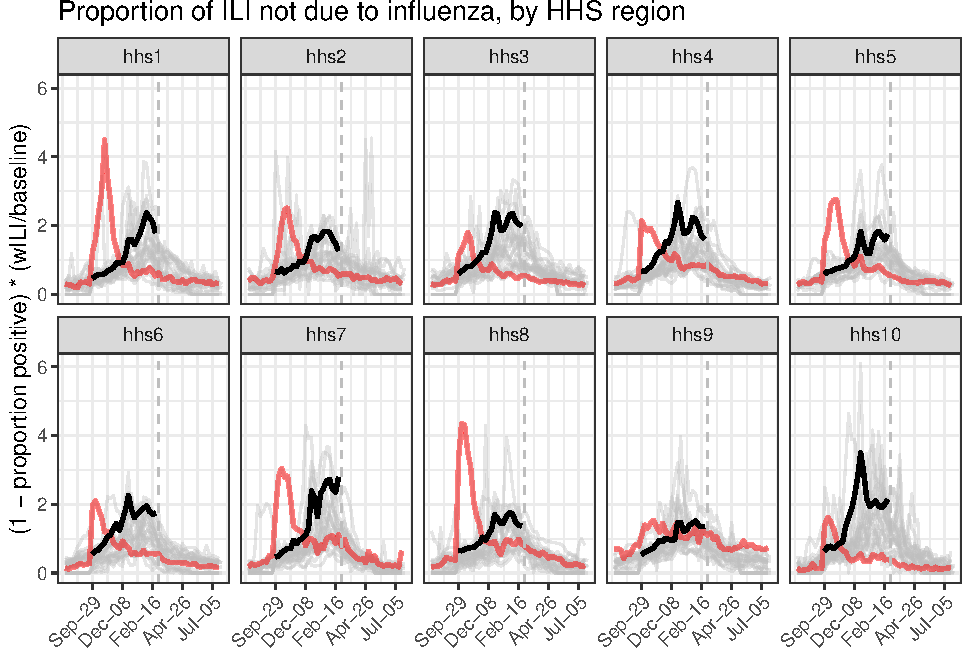
\includegraphics{ili-labtest-report_files/figure-latex/all-region-plot-ILI-1.pdf}
\caption{\label{fig:all-region-plot}US HHS Regions plots showing ILI-
values since the 2015/2016 season (top), and rILI- values (bottom).}
\end{figure}

\hypertarget{works-cited}{%
\subsection{Works Cited}\label{works-cited}}

{[}1{]}
\url{https://www.who.int/emergencies/diseases/novel-coronavirus-2019/situation-reports/}

{[}2{]} Yang, Y., Lu, Q., Liu, M., Wang, Y., Zhang, A., Jalali, N.,
Dean, N., Longini, I., Halloran, M. E., Xu, B., Zhang, X., Wang, L.,
Liu, W., \& Fang, L. (2020). Epidemiological and clinical features of
the 2019 novel coronavirus outbreak in China. MedRxiv,
2020.02.10.20021675. \url{https://doi.org/10.1101/2020.02.10.20021675}

{[}3{]} Imai, N., Cori, A., Dorigatti, I., Baguelin, M., Donnelly, C.
A., \& Riley, S. (n.d.). Report 3: Transmissibility of 2019-nCoV.
\url{https://www.imperial.ac.uk/media/imperial-college/medicine/sph/ide/gida-fellowships/Imperial-2019-nCoV-transmissibility.pdf}.

\hypertarget{changelog}{%
\subsection{Changelog}\label{changelog}}

16 February 2020: updated to revise name of COVID-19, updated case
counts and ILINet data, added citations and revised statements about R0.

2 February 2020: Updated to include new ILINet data released on Friday,
Jan 31.

26 January 2020: Although our overall assessment has not changed and our
analysis has not been updated, we have updated the discussion to better
convey the level of uncertainty in our analysis. We also added a heavier
line for the 2019/2020 season in the figures.

25 January 2020: First version of report released.


\end{document}
